% !TEX root = ../thesis.tex
\chapter{Sociological Research}
\label{chapter:sociological_research}
\thispagestyle{empty}

The aim of this chapter is to provide the reader with a sociological background by reporting information about gender gap in the society, overall at first and then with a focus on the U.S., which may be useful to understand and better contextualize the reasons behind the presence of possible preexisting biases and unequal gender representation in the results of our analysis.

We will start by providing information about the \textit{Global Gender Gap Index}, a powerful tool to measure different facets of the gender gap worldwide, and then we will focus on the U.S. by reporting some considerations about \textit{gender discrimination in the workplace}, taken from the literature in the field. Finally, some \textit{data and statistics from the U.S. Department of Labor} will be provided, with a brief comment on the displayed graphs.


\section{The Global Gender Gap Index}
A useful instrument to get a sociological overview on gender pay gap is provided by the World Economic Forum (WEF), ``an independent international organization committed to improving the state of the world by engaging business, political, academic and other leaders of society to shape global, regional and industry agendas'' \cite{world2021terms}. The World Economic Forum periodically releases a document -- The Global Gender Gap Report -- which contains information about gender-based inequalities in the various countries of the world, and provides a ranking based on a cumulative measure called \textbf{Global Gender Gap Index}, defined as:
\begin{quote}\emph{A framework for capturing the magnitude of gender-based disparities and tracking their progress over time. The Index benchmarks national gender gaps on economic, education, health and political criteria, and provides country rankings that allow for effective comparisons across regions and income groups.} \cite[p.~3]{schwab2017global}\end{quote}

The Index is based on three underlying criteria:
\begin{itemize}
\item It focuses on measuring \textit{gaps rather than levels}, because in this way the Index is disassociated from countries' levels of development, which would heavily impact on the results. For example, rich countries are able to offer more education and health opportunities to all members of society, but this is quite independent of the gender-related gaps that may exist within those higher levels of health or education \cite{schwab2017global}.
\item It captures \textit{gaps in outcome variables rather than gaps in input variables} (such as indicators related to country-specific policies, rights, or culture), in order to provide objective results based on fundamental measures related to basic human rights. For this reason, the Index relies on four categories (subindexes): Economic Participation and Opportunity, Educational Attainment, Health and Survival, Political Empowerment.
\item It ranks countries according to \textit{gender equality rather than women's empowerment}, because the focus is on the variation of the gap in the chosen indicators throughout the years. Therefore, the Index rewards countries that reach the point where outcomes for women equal those for men, but it neither rewards nor penalizes cases in which women are outperforming men.
\end{itemize}

The Global Gender Gap Report 2017 \cite{schwab2017global}, besides the mere ranking, provides some sociological interpretations of the results, based on the subindexes outcomes and on the parameters of which they are composed, such as the employee educational attainment by level, field of study, and gender, or the share and evolution of female hires in various industries. Although the majority of considerations are generic in nature, and not specific for the U.S. society, they are worth to be mentioned, since most of them could be reflected, on a small scale, in our case studies.
\begin{itemize}
\item There is a current stagnation of progress towards closing the economic gender gap, for several reasons:
\begin{itemize}
\item The global labor force participation has been in decline globally for both men and women, but this decline has been particularly accentuated for women.
\item Earned incomes of both men and women have been increasing, but this upward trend has been steeper for men than for women.
\item Women's share among senior positions both in the public sector and in business is not trending towards equal representation.
\end{itemize}
\item There is an under-use of the ever-increasing numbers of educated women because of discrepancies in caregiving and unpaid work, institutional and policy inertia, outdated organizational structures, and discrimination, but also skill differentials in the types of degrees women and men seek out in their education.
\item In many countries, a variety of social circumstances limit women's access to technology and therefore their ability to gain proficiency in its use. When women do have the relevant mathematical and technological skills, unconscious biases can influence their peers' recognition of their capabilities.
\item There exist imbalances in the specific fields of study in which men and women tend to specialize. Women are underrepresented in the engineering, manufacturing, and construction as well as information, communication, and technology fields.
\item There is a tendency towards lower pay for occupations that have historically developed as predominantly female. When women enter a profession in large numbers, the pay-related benefits of participating in the profession depreciate.
\item The female leadership representation remains below 50\% in all industries, and every industry exhibits a leadership gender gap.
\item Unconscious biases and systemic efforts focused on driving change at the industry or country level through public-private collaboration remain scarce.
\end{itemize}

Appendix~\ref{appendixA} shows the country profile of the United States in the report. As we can see, the country was ranked 49th out of 144, with an overall score of 0.718 (in a score system in which 1 means gender parity), and Political Empowerment is the subindex in which the U.S. performed worst. For the purpose of our research, it is particularly useful to look at the \textit{Economic participation and opportunity} section of the country score card, in which we can notice that men are more participatory in the labor force than women, and women tend to earn less then men for similar jobs. Furthermore, the estimated earned income for women is significantly lower than the one of men, and the last two items show that women are underrepresented in managerial positions and higher-paying jobs, and are overrepresented in professional and technical works. From the \textit{Workforce Participation} section of the selected contextual data we can see that women are more likely than men to be employed part-time, and also not to be paid for their work.

Other considerations about the gender gap, as depicted in The Global Gender Gap Report 2017, are done by the authors of \cite{hazel2019gender}. Even if the most relevant for us are the ones concerning the Economic Participation and Opportunity subindex, we believe that for a broader understanding it is worth to briefly report also the main points related to the other subindexes, especially because they have an impact on the condition of women which can also affect the workplace:
\begin{itemize}
\item \textbf{Economic Participation and Opportunity}: women seem to be more likely than men to be living at or below poverty, mainly because of the following reasons:
\begin{itemize}
\item Many women remain economically dependent on men.
\item Women are more likely than men to be unemployed or to work in positions in which they do not get paid.
\item Women are more likely than men to be concentrated in industries and occupations with low wages, long hours, and no social protections, and less likely than men to hold management positions.
\item Women in general earn only 82\% compared to white men, and the gender wage gap becomes further complicated when race/ethnicity is taken into account.
\end{itemize}
\item \textbf{Educational Attainment}: women are concentrated in traditionally female and lower-paying CTE (Career and Technical Education) programs in both secondary and postsecondary educational settings, and are still underrepresented in Science, Technology, Engineering, and Math (STEM) programs. Gender stereotypes and bias in education and the potentially hostile climate of academic departments continue to deter women from these lucrative career opportunities.
\item \textbf{Health and Survival}: women are at a disadvantage compared to men, mainly because of the following reasons:
\begin{itemize}
\item Poor access to information, early marriage, lack of decision-making power continue to increase women's exposure to sexually transmitted diseases, unwanted pregnancies and the risk of unsafe abortions.
\item Women are constantly bombarded with media advertisements that sexualize their bodies. The influence of media, television, movies, etc. has led to increased prevalence of body dissatisfaction and eating disorders globally.
\item Violence towards women continues to impact women's health worldwide, and makes it difficult for women to pursue educational opportunities or to perform their jobs.
\end{itemize}
\item \textbf{Political Empowerment}: women hold a minority of political and institutional decision-making positions. Gender norms and prejudices work to both reduce the number of female candidates and contribute to the obstacles faced by women in elections.
\end{itemize}

Finally, we believe it is worth to mention that the Global Gender Gap Index is not the only tool to evaluate gender equality among countries, and another example is represented by the \textit{Historical Gender Equality Index (HGEI)}, introduced in \cite{dilli2018introducing}. As the name itself suggests, HGEI is based on some historical measures, since gender inequality is strictly related to the human history, and it has the aim of providing a global overview of gender equality in the long run, as well as to give an indication of gender disparities in well-being outcomes that result from institutional, cultural, and social influences.
Similarly to the Global Gender Gap Index, HGEI is also based on a few requirements -- coverage (of gender equality dimensions), availability of data for many countries, simplicity in calculation and understanding, possibility of comparisons between countries but also over time -- and it is a composite index made of four dimensions -- health, autonomy within the household, political power, socioeconomic status -- each of which composed by some indicators.
As the Global Gender Gap Index, also HGEI is based on ratios rather than levels, in order to evaluate the position of women relative to men in each society rather than the actual levels of resources and opportunities available to women, and therefore it does not capture how women are doing in absolute terms, and it cannot show if there are cases where women are outperforming men.
HGEI revealed that most countries of the world made progress toward gender equality over the past fifty years, but there is little convergence between them, and the authors recommend that future research should also pay attention to the dimensions in which gender inequality occurs, because behind a composite index can lie great variation in the underlying indicators.


\section{Gender Discrimination in the Workplace}
The Global Gender Gap Index is a powerful indicator, which provides us with an overview on the main fields in which women experience inequalities, particularly on a large scale, and with some sociological motivations for these disparities. We will now focus on some literature regarding the U.S. society and more specific on the labor market.

Tilcsik in \cite{tilcsik2021statistical} brings into play the theory of \textbf{statistical discrimination}, which rather than merely explaining discrimination, helps rationalize and justify discriminatory decisions. As reported in the article:
\begin{quote}\emph{This theory \emph{[statistical discrimination]} posits that employers have imperfect information about the future productivity of job candidates, which gives them an incentive to use easily observable ascriptive characteristics, such as race or gender, to infer the expected productivity of applicants. \emph{[\ldots]} In this model, discrimination does not arise from animus or antipathy toward members of a group; rather, it is portrayed as a rational solution to an information problem.} \cite[p.~94]{tilcsik2021statistical}\end{quote}

Statistical discrimination is in contradiction with the other dominant economic perspective on discrimination, known as \textbf{taste-based model}:
\begin{quote}\emph{Unlike statistical discrimination theory, which taps into the culturally valued discourse of instrumental rationality and frames discrimination as a logical solution to an information problem, the taste-based model is about negative attitudes, such as overt racial prejudice and sexism, that tend to be publicly disavowed and are often perceived as socially unacceptable.} \cite[p.~95]{tilcsik2021statistical}\end{quote}

Tilcsik focused on some sociological perspectives in support of the statistical discrimination theory, explaining that status beliefs and stereotypes shape how employers evaluate workers and how they distribute rewards among them. Indeed, when employers are required to evaluate groups of candidates for a job position, their perceptions of the differences among the groups reflect cultural beliefs that are often inaccurate and resistant to change, even in the face of disconfirming evidence, and therefore it is not a matter of intentional discrimination but of societal bias.

Statistical discrimination is likely to have some resonance and normative acceptability for three main reasons \cite{tilcsik2021statistical}:
\begin{itemize}
\item It is a rational, profit-maximizing, incentive-driven decision, and represents `the optimal solution to an information extraction problem'.
\item Some economists characterize it as fair and morally defensible, by implying that categorical differences are rooted in statistical considerations that rational employers consider, and by suggesting that statistical discrimination is fair and neutral because it treats people with the same expected productivity identically.
\item Economists often emphasize that it is ubiquitous and practically inevitable in many domains of life.
\end{itemize}
Thus, the use of stereotypes is depicted as cognitively and economically useful as well as consistent with social norms. Exposure to the idea of statistical discrimination strengthen people's belief in the validity, usefulness, and acceptability of relying on stereotypes and hence increase their likelihood of engaging in discrimination because of ascriptive group characteristics. When employers feel confident that their decisions are impartial, rational, and ethically defensible, they feel more justified in relying on stereotypes and exert less effort to suppress their biases. Statistical discrimination may also become self-fulfilling if it leads members of negatively stereotyped groups to believe that investing in their skills will not be fully rewarded.

Tilcsik in \cite{tilcsik2021statistical} also conducted a a survey experiment consisting in a hiring simulation, in which participants (who all had managerial experience) were randomly assigned to one of four conditions:
\begin{itemize}
\item[1.] Exposure to statistical discrimination theory (treatment).
\item[2.] No exposure to any theory of discrimination (non-treatment).
\item[3.] Exposure to the taste-based model (placebo).
\item[4.] Exposure to statistical discrimination theory and a critical commentary (treatment variant).
\end{itemize}
Participants exposed to the theory (without a critical commentary) perceived stereotyping as more acceptable and stereotypes as more accurate than did participants in the other groups, and selected fewer women for their teams. Group representation was also impacting on decisions, since female participants and those who did not identify as either male or female were, on average, less convinced of the acceptability and accuracy of stereotypes than were male respondents.

Beggs in \cite{beggs1995institutional} instead shifts the focus on the impact of the \textbf{institutional environment} on gender and race inequalities in the labor market. According to the theoretical background he depicts, ``organizations compete not just for resources and customers, but for political power and institutional legitimacy, for social as well as economic fitness'' \cite[p.~613]{beggs1995institutional}, from \cite[p.~150]{dimaggio1983iron}. Therefore, an important factor to consider is the force of public opinion: when new definitions or practices become legitimated and accepted, organizations are under considerable pressure to incorporate them.

Beggs decided to analyze data from the 1980 U.S. Census in order to prove the two hypotheses reported below \cite{beggs1995institutional}:
\begin{itemize}
\item[1.] Within industries, the higher the proportion of workers employed in states with high support for equality, the lower the levels of race and gender inequality in jobs and earnings.
\item[2.] The higher the proportion of federal public sector employees in an industry, the lower the levels of race and gender inequality in jobs and earnings.
\end{itemize}

For the analysis, he decided to adopt some measures, each of which composed by several indicators: local institutional environment and national institutional environment (independent variables), quality of employment and earnings inequality (dependent variables), industrial structure, human capital inequality, and employment inequality (control variables).

According to his results, the institutional environment impacts both quality of employment and earnings. For what concerns the former, greater support for equality in the local institutional environment, as well as greater federal public sector employment in an industry, is associated with lower levels of inequality among minorities (race/gender groups). As for the latter, the greater the support for equality in the local institutional environment, the better the earnings position of each minority relative to white men, and the level of federal public sector employment in an industry is positively associated with the earnings position of all minorities.

Finally, an interesting point of view is provided in \cite{folbre2021gender}, a report published by the Economic Policy Institute. Folbre highlights that women in the U.S. still tend to earn 20\% less per hour than men, and points out that empirical research on the causes of the persistent earnings gap often takes the form of statistical models that control for as many variables as possible (such as race, education, labor force experience), but control variables cannot be explained purely as the result of individual choices. Rather, they reflect structural inequalities related to \textbf{unequal bargaining power}.
\begin{quote}\emph{Bargaining often characterizes situations where two parties, whether individuals or groups, see potential gains from cooperation but disagree over how those gains should be shared. Both parties can potentially benefit from coming to an agreement, and their share is likely to be strongly affected by their fallback position, or next-best option.} \cite[p.~9]{folbre2021gender}\end{quote}

We can summarize the main points of Folbre's research (that is, the main causes of gender gap) as follows:
\begin{itemize}
\item \textbf{Stereotypes}: in the U.S. women who move into better paying but stereotypically masculine occupations often face sexual harassment and disapproval. When wives earn more than husbands, both spouses slightly tilt their reported earnings to conform to gender stereotypes, overstating the relative size of husbands' earning.
\item \textbf{Pay penalties}: many women self-select into traditionally female occupations because they consider these more compatible with the demands of family care. But while they may be aware that these jobs pay less than traditionally male jobs, they do not choose the size of the resulting pay penalties: in the U.S. the percentage of women in an occupation is inversely related to its average pay, even controlling for human capital characteristics.
\item \textbf{Mothers discrimination}: many women experience wage penalties because of becoming mothers. Discrimination against mothers is based on rather subtle cues, such as participation in a parent-teacher organization listed on a job resume, because employers may assume that mothers of young children face other demands on their time that lower their performance in paid employment.
\item \textbf{Mobility}: women's labor supply is less elastic than men's because women's mobility between jobs is limited by obligations of family care. Employers can easily take advantage of this difference, paying women less than men not because they prefer hiring men but because they recognize that women are more likely to accept lower wages.
\item \textbf{Occupational segregation}: high levels of occupational segregation are still the largest immediate cause of gender inequality in earnings. Efforts to improve the relative pay of primarily female jobs met criticism based on the assumption that occupational pay was largely determined by productivity. Finally, the supply of women's labor to the market was treated merely as the result of individual choices, with little attention to the constraints imposed by a traditionally male-oriented organization of work, school, housework, and childcare.
\item \textbf{Information asymmetries}: employers are often able to use their control over information to lower women's wages relative to men's, because not all the workers are covered by the Fair Labor Standards Act (which guarantees the right of workers to discuss their salaries), and others remain unaware of their rights. Furthermore, employers in most states have the right to ask job applicants what they earned in their previous jobs and to adjust wage offers accordingly. For this reason, women's entrance into previously male-dominated occupations tends to lower the average occupational wage, and this `devaluation' is at least partially driven by the fact that women start out in lower-paying (often part-time) occupations, which lowers their bargaining power.
\item \textbf{`Equal value' principle}: whatever a worker is paid represents his or her value added -- therefore, men earn more than women because they contribute more to society. Unfortunately, this principle does not take into account that many female-dominated services have a public good dimension: their social value exceeds their private value. The work of caring for others creates value that is difficult to capture through the market because it often involves emotional engagement, teamwork, and person-specific skills. Women's tendency to devote more hours to unpaid care work than do men is interpreted because of feminine preferences rather than as the result of institutional pressure to ensure a generous supply of female effort to activities such as family care that cannot be rewarded by market forces.
\item \textbf{Paid work/family work constraints}: responsibility for the care of family, friends, and neighbors weighs more heavily on women than men, not because women necessarily prefer this arrangement but because men often have sufficient bargaining power to minimize demands on their time. Furthermore, women labeled as uncaring are typically stigmatized, and employers use this social norm to justify lower pay offers to women.
\end{itemize}


\section{Data \& Statistics (U.S. Department of Labor)}
\label{section:data_statistics_dol}
The last step of our sociological research consists in the reporting of some interesting data and statistics\footnote{Available at: \url{https://www.dol.gov/agencies/wb/data}.} taken from the U.S. Department of Labor, and more specifically from Women's Bureau, an agency within the Department with the aim of developing policies and standards and conducting inquiries to safeguard the interests of working women, to advocate for their equality and economic security for themselves and their families, and to promote quality work environments.

\begin{figure}[t!]
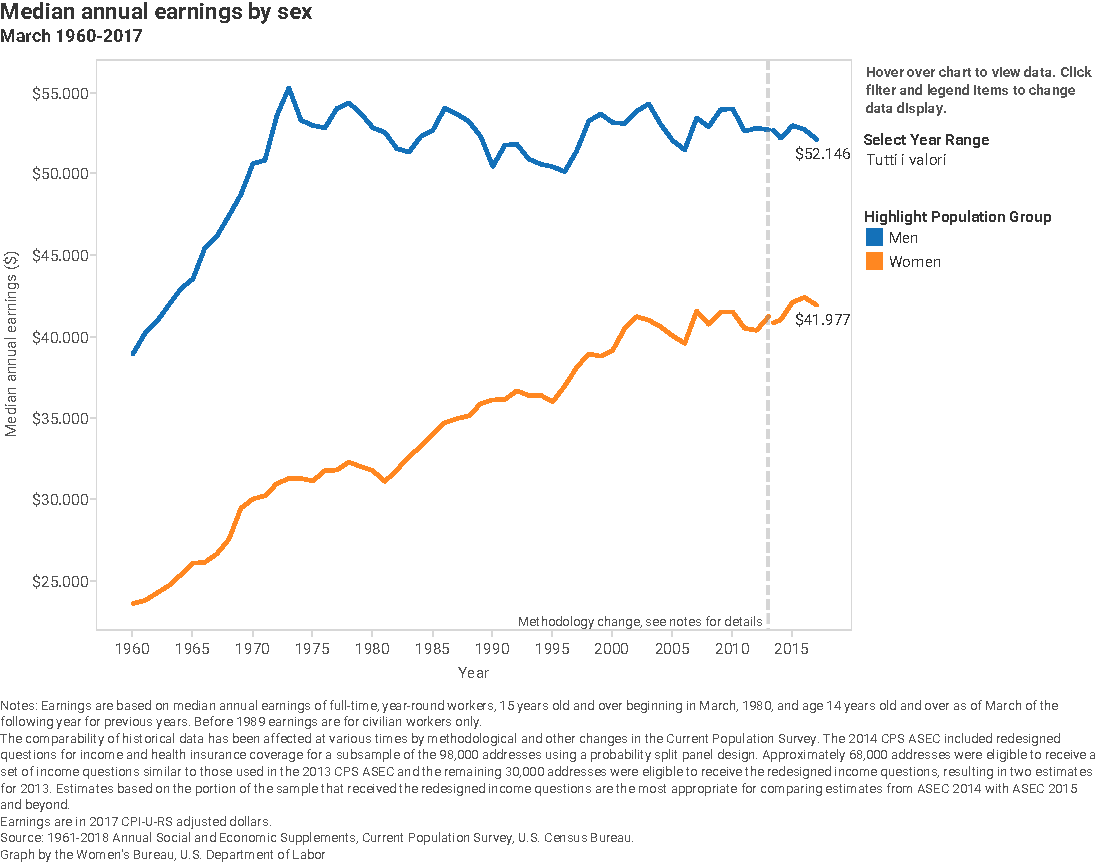
\includegraphics[scale=.7]{figures/dol_earnings_by_sex.pdf}
\centering
\caption{Median annual earnings by sex (1960--2017).\newline
U.S. Department of Labor. Source: \upshape\protect\url{https://www.dol.gov/agencies/wb/data}.}
\label{fig:dol_earnings_by_sex}
\end{figure}

First of all, Figure~\ref{fig:dol_earnings_by_sex} shows that, since 1960, both male and female earnings increased by about \$15K, but, because of the large initial gap, the actual average incomes still differ by about \$10K in favor of men. Furthermore, the graph does not take into account part-time workers, the introduction of which would lead to an accentuation of the gap between men and women, since, as Figure~\ref{fig:dol_full-_and_part-time_workers_by_sex} displays, most part-time workers are women (over 60\% of the total number of part-time employees).

\begin{figure}[t!]
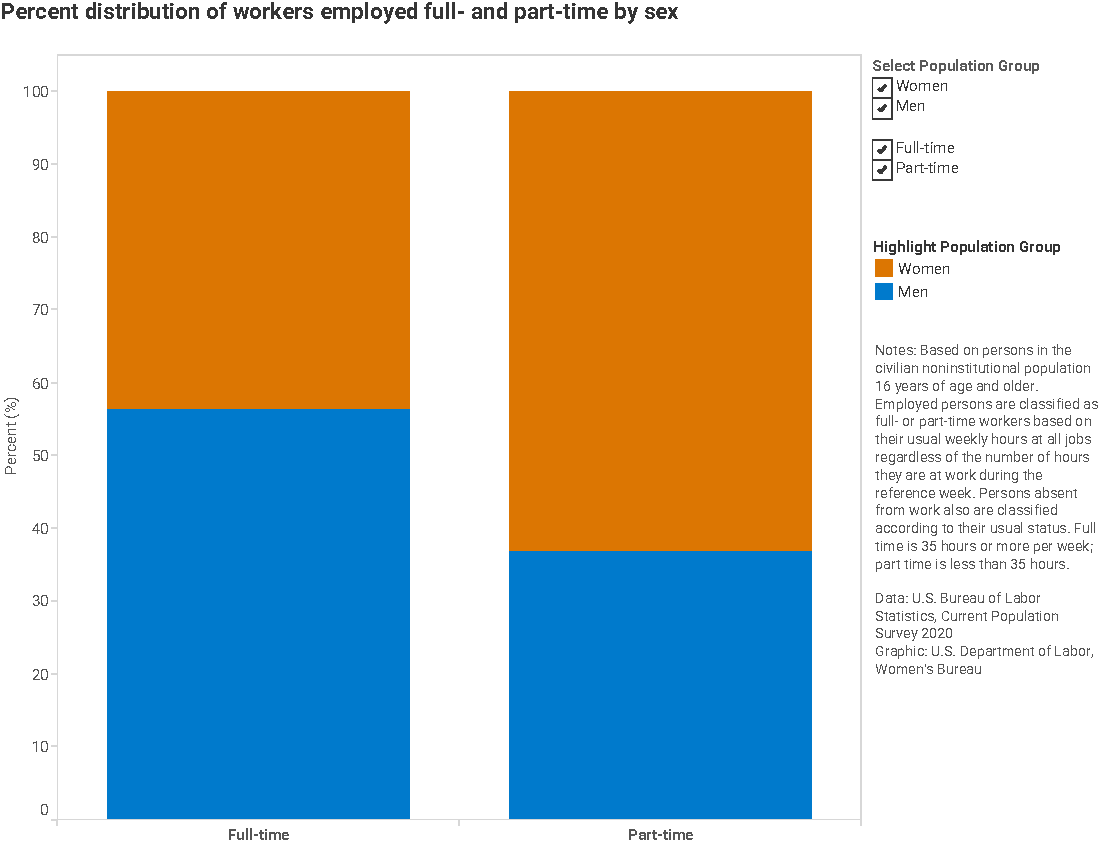
\includegraphics[scale=.7]{figures/dol_full-_and_part-time_workers_by_sex.pdf}
\centering
\caption{Percent distribution of workers employed full- and part-time by sex (2020).\newline
U.S. Department of Labor. Source: \upshape\protect\url{https://www.dol.gov/agencies/wb/data}.}
\label{fig:dol_full-_and_part-time_workers_by_sex}
\end{figure}

\begin{figure}[t!]
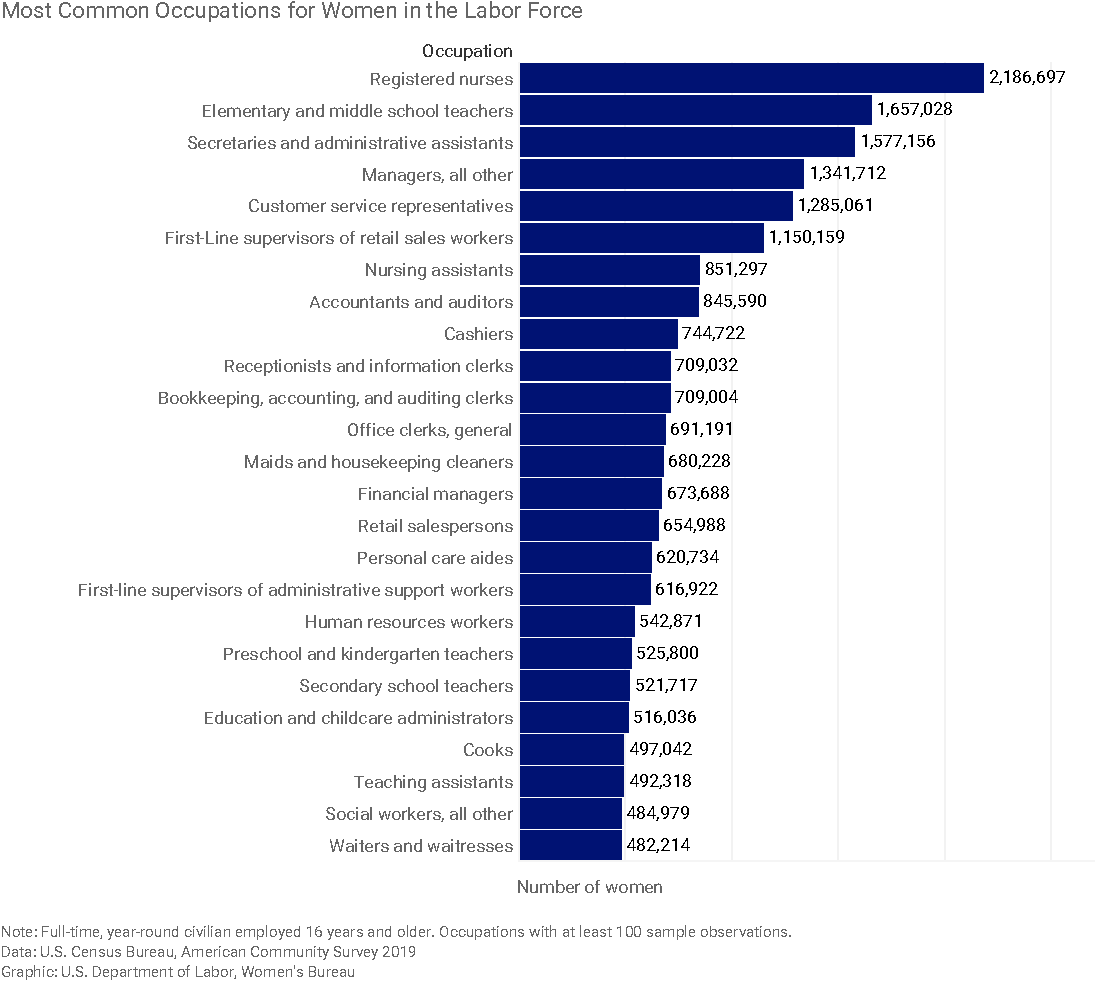
\includegraphics[scale=.7]{figures/dol_most_common_occupations_women.pdf}
\centering
\caption{Most common occupations for women in the labor force (2019).\newline
U.S. Department of Labor. Source: \upshape\protect\url{https://www.dol.gov/agencies/wb/data}.}
\label{fig:dol_most_common_occupations_women}
\end{figure}

Figure~\ref{fig:dol_most_common_occupations_women} shows the most common occupations for women. As we can see, in accordance with the other sociological sources, the podium is constituted by nurses, teachers, and secretaries. The representation problem is even exacerbated when looking at Figure~\ref{fig:dol_occupations_over_time}, which is interesting for us because it displays the top-10 occupations employing the largest number of women for the same year without excluding part-time employees. Even though data are a bit more aggregated (for example, the teachers category presumably includes not only elementary and middle school teachers), the numbers, in comparison with Figure~\ref{fig:dol_most_common_occupations_women}, dramatically increase, emphasizing again the huge percentage of women working part-time. This problem is particularly accentuated for some job titles, typically not very profitable (such as cashiers and waitresses), which overcome more advantageous positions (like managers) in the list. Figure~\ref{fig:dol_stem_percent_women} instead highlights again how women are underrepresented in STEM disciplines, especially in computer occupations and engineering. Although the trend is generally increasing, the rate of increase is very low (+4\% in 30 years, from 1990 to today), and it is particularly dramatic to observe the decrease in the percentage of female employees working in computer occupations, which had a peak -- never reached again -- back in 1990.

\begin{figure}[t!]
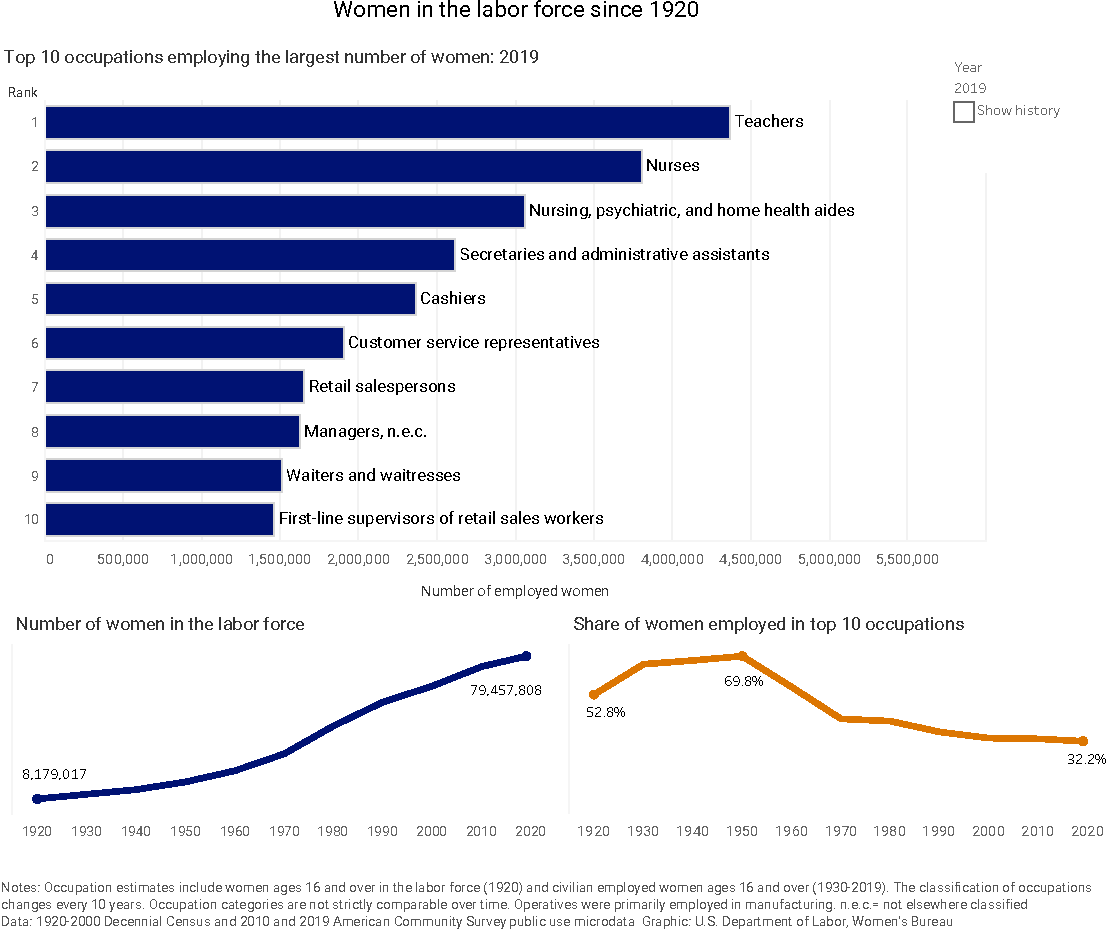
\includegraphics[scale=.7]{figures/dol_occupations_over_time.pdf}
\centering
\caption{Top-10 occupations employing the largest number of women (2019).\newline
U.S. Department of Labor. Source: \upshape\protect\url{https://www.dol.gov/agencies/wb/data}.}
\label{fig:dol_occupations_over_time}
\end{figure}

\begin{figure}[t!]
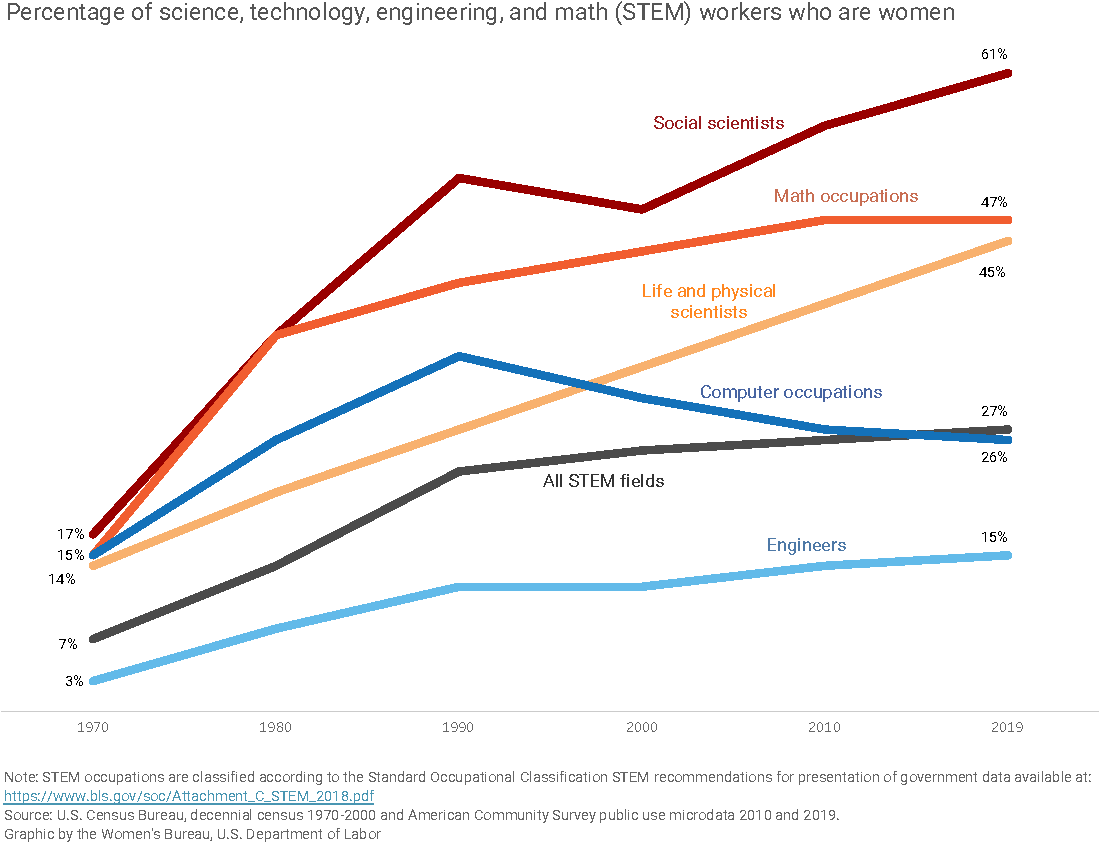
\includegraphics[scale=.7]{figures/dol_stem_percent_women.pdf}
\centering
\caption{Percentage of Science, Technology, Engineering, and Math (STEM) workers who are women (1970--2019).\newline
U.S. Department of Labor. Source: \upshape\protect\url{https://www.dol.gov/agencies/wb/data}.}
\label{fig:dol_stem_percent_women}
\end{figure}

Finally, Figure~\ref{fig:dol_occupations_with_largest_gender_earnings_gap} displays the ordered list of occupations with the largest gender earnings gap. Most of the professions are traditionally lower-paying jobs, and no STEM or managerial disciplines appear to be listed. As a consequence, considering the lower percentage of women employed in STEM and managerial positions, and considering that in general most part-time workers are employed in lower-paying jobs, we can put emphasis on the percentage of women being disadvantaged in comparison with men, and on the still present significance of the gender gap.

\begin{figure}[t!]
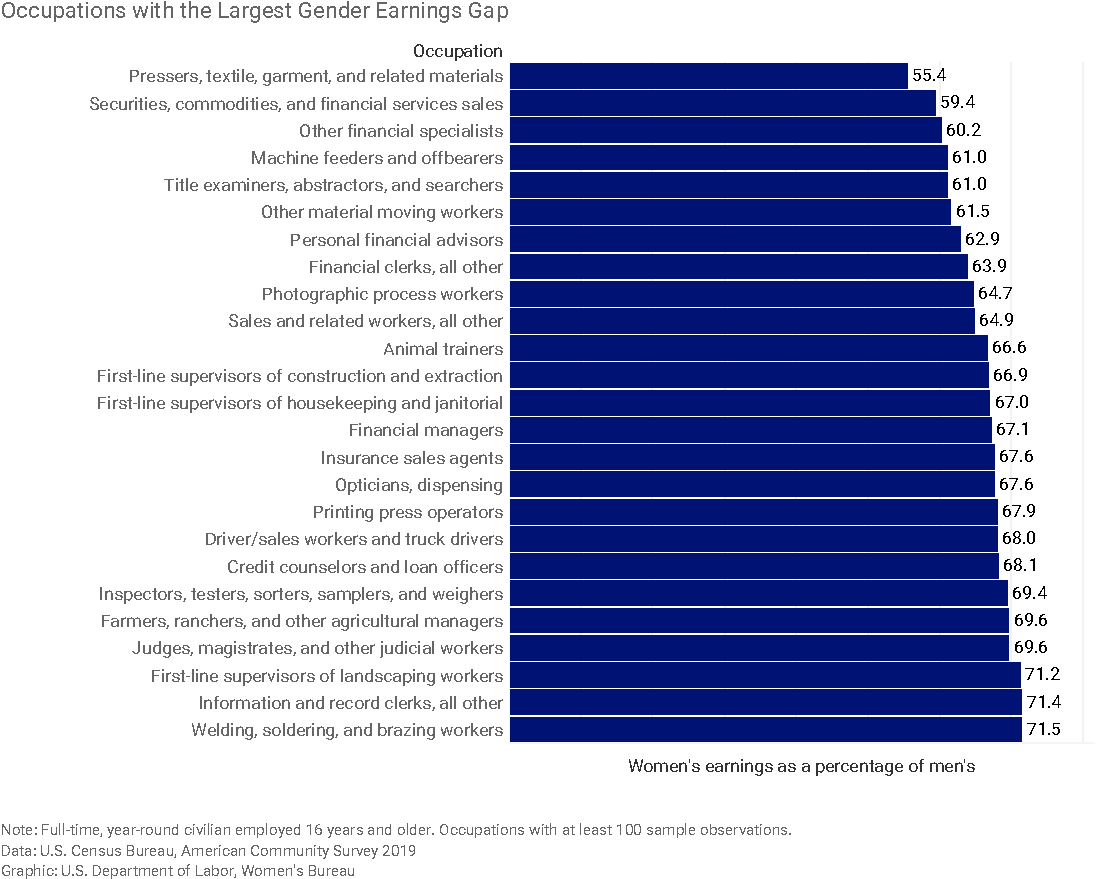
\includegraphics[scale=.7]{figures/dol_occupations_with_largest_gender_earnings_gap.pdf}
\centering
\caption{Occupations with the largest gender earnings gap (2019).\newline
U.S. Department of Labor. Source: \upshape\protect\url{https://www.dol.gov/agencies/wb/data}.}
\label{fig:dol_occupations_with_largest_gender_earnings_gap}
\end{figure}
